%%%%%%%%%%%%%%%%%%%%%%% file template.tex %%%%%%%%%%%%%%%%%%%%%%%%%
%
% This is a general template file for the LaTeX package SVJour3
% for Springer journals.          Springer Heidelberg 2010/09/16
%
% Copy it to a new file with a new name and use it as the basis
% for your article. Delete % signs as needed.
%
% This template includes a few options for different layouts and
% content for various journals. Please consult a previous issue of
% your journal as needed.
%
%%%%%%%%%%%%%%%%%%%%%%%%%%%%%%%%%%%%%%%%%%%%%%%%%%%%%%%%%%%%%%%%%%%
%
% First comes an example EPS file -- just ignore it and
% proceed on the \documentclass line
% your LaTeX will extract the file if required
\begin{filecontents*}{example.eps}
%!PS-Adobe-3.0 EPSF-3.0
%%BoundingBox: 19 19 221 221
%%CreationDate: Mon Sep 29 1997
%%Creator: programmed by hand (JK)
%%EndComments
gsave
newpath
  20 20 moveto
  20 220 lineto
  220 220 lineto
  220 20 lineto
closepath
2 setlinewidth
gsave
  .4 setgray fill
grestore
stroke
grestore
\end{filecontents*}
%
\RequirePackage{fix-cm}
%
\documentclass{svjour3}                     % onecolumn (standard format)
%\documentclass[smallcondensed]{svjour3}     % onecolumn (ditto)
%\documentclass[smallextended]{svjour3}       % onecolumn (second format)
%\documentclass[twocolumn]{svjour3}          % twocolumn
%
\smartqed  % flush right qed marks, e.g. at end of proof
%
\usepackage{mhsetup}
\usepackage{amsmath}
\usepackage{mathtools}
\usepackage{natbib}
\usepackage{graphicx}
\usepackage{float}
\usepackage{qtree}
\usepackage[utf8]{inputenc}
\usepackage{gb4e}
\usepackage[T1]{fontenc}
\usepackage{ tipa }
\usepackage{hyperref}
\usepackage{soul}
\bibpunct[: ]{(}{)}{,}{a}{}{,}
\newcommand{\noteme}[1]{\noindent \textbf{[[JCW:  #1 ]]}}
\renewcommand{\theequation}{\Alph{equation}}

% Insert the name of "your journal" with
\journalname{Journal of }

\begin{document}

\title{Extraposition is Disapppearing
\thanks{I'd like to thank Josef Fruehwald, Anthony Kroch, Caitlin Light, and Gary Thoms for very helpful discussion on this and related topics, as well as audiences at the Diachronic Generative Syntax Conferences in 2013 and 2014, and at seminar series' at University College London and the University of Geneva for comments on earlier versions of some of this material. I'd also like to particularly thank George Walkden for his comments on a pre-final draft, and three anonymous reviewers. All errors are my own.}}
%\subtitle{Do you have a subtitle?\\ If so, write it here}

%\titlerunning{Short form of title}        % if too long for running head

\author{Joel C. Wallenberg}

%\authorrunning{Short form of author list} % if too long for running head

\institute{Joel C. Wallenberg \at
              Newcastle University \\
              Tel.: +44-(0)191-222-7366\\
              \email{joel.wallenberg@ncl.ac.uk}
}

\date{Received: date / Accepted: date}
% The correct dates will be entered by the editor


\maketitle

\begin{abstract}
This study describes a change in which relative clause extraposition is in the process of being lost in English, Icelandic, French, and Portuguese. This current change in progress has never been observed before, probably because it is so slow that it is undetectable without the aid of multiple diachronic parsed corpora (treebanks) with time-depths of over 500 years each. In fact, building on insights from \citet{kiparsky1995}, the change may date as far back as the innovation of Proto-Germanic and Proto-Romance relative clauses, as these varieties differentiated from Proto-Indo-European. The study also shows that the unusually slow speed of the change is due to partial specialization of the construction along the dimension of prosodic weight, following the argument made at greater length in \citet{fruehwaldwallenberginprep}. Finally, the change is shown to have important consequences for the syntax of extraposition, supporting the adjunction analysis of \citet{culicoverrochemont1990}. The paper also discusses the implications of \citet{sauerland2003} analysis of English relative clauses, and while modern English data supports his analysis, the diachronic extraposition data is not yet fine-grained enough to bear on the ``raising'' analysis of relatives in general. This is identified as an important question for further research on this change.
\keywords{syntax \and language change \and Indo-European \and evolutionary dynamics \and treebanks}
% \PACS{PACS code1 \and PACS code2 \and more}
% \subclass{MSC code1 \and MSC code2 \and more}
\end{abstract}

\section{Introduction}
\label{intro}
%Kiparsky 1995, Hopper (Hooper?) & Traugott 200?
This squib presents important preliminary results demonstrating the existence of a syntactic change which is many times slower than any other that has previously been reported: relative clause extraposition is being lost in both Germanic and Romance languages.
%Depending on what is driving the change, it may also be a new class of syntactic change. 

Furthermore, this decline in extraposition has been underway for over a thousand years, and while it is nearing completion in modern Portuguese, the change appears to still be ongoing at the present time.
As the results are still preliminary and much of their analysis is still unclear, the main goal of this article is to carefully describe a type of syntactic change which presents problems for both synchronic syntactic theory and the theory of language change, but not to present a comprehensive analysis of every aspect of this change, or this construction, at the present time. I hope this will be the first of many studies of this interesting and important phenomenon, and I consider the suggestions here to be a starting point, not anything near the last word on the subject.

This is to say that the construction exemplified in (\ref{construct1}) is currently in decline, and possibly on a slow path to extinction:

\begin{exe}
    \ex %English (constructed):
    \begin{xlist}
         \ex \label{construct1} Another method...may be employed which is less open to the above objection.\\
         (John Strutt's Scientific Papers, date: 1890; STRUTT-1890,3,356.396 in \textsl{Penn Parsed Corpus of Modern British English}, \citealt{ppcmbe})\\
         \ex \label{construct2} Another method which is less open to the above objection may be employed\\
         (Constructed)
        \end{xlist}
\end{exe}

To define the scope of enquiry more precisely, this study considers the extraposition of finite relative clauses, CP-sized clauses containing a gap, where the gap is interpreted as referrring to some NP antecedent. (The antecedent is standardly referred to as the ``relative head'', even though it's not a head at all, in the technical sense.) The extraposed relatives this study considers are where the entire finite clause containing the gap is displaced from the ``relative head'', whether this is analyzed as movement or something else, surfacing at the right edge of the $v$P or higher TP. (A more detailed description of how these are located in the historical corpora can be found in section \ref{methods}.) Extraposed relatives have often been analyzed as an instance of rightward movement followed by right-adjunction, but they have also been analyzed (following \citealt{kayne1994}) as being the result of the leftward movement of other material (see \citealt{baltin2006} for an overview of various analyses and their shortcomings). We will be particularly concerned with extraposed relatives that are interpreted with respect to an NP in the subject of the higher clause, as in (\ref{construct1}), though some data on extraposition from objects will also be presented.

The goal of this paper is to present some potentially important preliminary findings, and some possible interpretations of those findings; the goal is not to present the definitive analysis of extraposition, or of the diachronic change. That being said, the simple result this article presents, that extraposed relatives are in decline, has the following consequence: any analysis of relative clauses (and extraposition) must take into account the fact that the extraposed and \textsl{in situ} variants are, in some sense, ``competing grammars'' \citep[in the sense of][inter alia]{kroch1989, kroch1994}; they must be in competition in language use, as one variant is in the process of replacing the other.
The fact that such slow changes exist, and that their effects on synchronic language use can be demonstrated, should cause all researchers in synchronic syntax to question whether all purported cases of ``optional'' movements are in fact changes in progress.
Perhaps ``optional'' has no coherent meaning in grammar, outside of the meaning of change in progress.

The paper is organised as follows.
First, I report quantative data that relative clause extraposition is being lost in the following languages: English, Icelandic, French, and Portuguese, using seven different parsed diachronic corpora (i.e. treebanks).
Next in \ref{compete}, I discuss the idea that the extraposed and \textsl{in situ} variants are ``competing grammars'', syntactic variants which are mutually exclusive and competing in language use, and suggest some consequences this has for the analysis of relative clauses. In particular, I consider whether the competing grammars we see could be the competing structures for relative clauses identified by \citet{sauerland2003}, and/or whether they are competing adjunction sites, building on \citet{culicoverrochemont1990}.
In section \ref{slow}, I discuss the fact that the extraposed variant is specialized for particularly heavy relative clauses, which is the factor that slows the change down to a degree that it is only observable over a period of a thousand years.
Finally, section \ref{pie} builds on \citet{kiparsky1995} and presents the possibility that this change began back in pre-history, at a time when true relative clauses were first innovated in Romance and Germanic, and has been underway ever since.



\section{Decline in Relative Clause Extraposition}
\label{relclause}

The data in \ref{results} below show a remarkably slow decline in the frequency of relative clause extraposition from subject DPs in four languages: English, Icelandic, French, and Portuguese. I originally collected this data to test the hypothesis that the frequency of relative clause extraposition was stable over time in a number of languages; as you will see below, though the change is slow enough to be unobservable without data from over a period of many hundreds of years, that hypothesis can be soundly rejected.

\subsection{Methods}
\label{methods}

It is worth noting that the type of data presented below is entirely unobtainable without diachronic parsed corpora (i.e. treebanks), which have been annotated at a very high level of accuracy (i.e. they have been hand-corrected by expert syntacticians, not only automatically parsed). For this study, the following parsed diachronic corpora were used: for English, the \textsl{York-Toronto-Helsinki Corpus of Old English Prose (YCOE)} \citep{ycoe}, the \textsl{Penn-Helsinki Parsed Corpus of Middle English 2 (PPCME2)} \citep{ppcme2}, the \textsl{Penn-Helsinki Parsed Corpus of Early Modern English (PPCEME)} \citep{ppceme}, and the \textsl{Penn Parsed Corpus of Modern British English (PPCMBE)} \citep{ppcmbe}; for Icelandic, the \textsl{Icelandic Parsed Historical Corpus (IcePaHC)} \citep{icepahc09}; for Old and Middle French, the \textsl{MCVF Corpus} \citep{mcvf}; and for historical Portuguese, the \textsl{Tycho Brahe Corpus of Historical Portuguese} \citep{tychobrahe}.

Finite clauses containing a relative clause modifying a subject or object were extracted from the corpora using CorpusSearch coding queries \citep{corpussearch}, and coded for the following variables: the response variable of whether or not the relative clause was extraposed, whether it modified a subject or object DP, its weight in number of words, whether the clause occurred in reported speech or not, and the date of the text the clause appeared in.\footnote{If no precise date of composition was available, as was the case for many Old English and Old Icelandic texts, we used an estimated date of composition wherever possible, or a manuscript date in cases where there is no clear consensus on the date of composition. In all cases, we follow the dates provided by the documentation of the diachronic corpora, following the philological sources they cite.} These variables were controlled for in all subsequent statistical analysis. Extraposed finite relatives are annotated in the same way across all of the corpora above, as a ``CP-REL'' inside of an NP, which dominates a particular kind of trace, labelled ``ICH''. The trace is coindexed with another ``CP-REL'' node that occurs displaced from the trace position, to the right of some other clause-level material. This annotation is only given when the relative unambiguously has a gap corresponding to some ``relative head'' NP, and when the relative is clearly displaced from that NP in the string. (Please see the annotation manuals for the corpora, and my actual queries, for more detail.)

%åFor English, Icelandic, and Portuguese, only prose texts are 

All coding queries and the extracted datasets are available at in the following public \textsl{git} directory: \url{github.com/joelcw/tyneside/tree/master/extraposition/queriesandoutput}.
%were coded so that the effects of these variables could be controlled for in statistical analysis.



%agnostic as the rightward/leftward-movement question
%Cite Anton about phonological weight being continuous, not discrete !!!


%extraposition in modern Dutch and German, which has specialized along a grammatical, categorical dimension

\subsection{Results}
\label{results}

For the four languages I investigated, English, Icelandic, French, and Portuguese, there is a slow but steady decline in the rate of relative clause extraposition over the course of each language's written history (given the corpora we currently have), compared to the use of \textsl{in situ} relative clauses. This is shown in Figures \ref{engfig}-\ref{portfig}. (For data sets in the form of lists of codes extracted from the corpus, please see files ending in ``.ooo'' in the github directory linked above, i.e. \url{github.com/joelcw/tyneside/tree/master/extraposition/queriesandoutput/*.ooo}. The code lists are easily importable into R, and same directory contains queries, ending in ``.c'', which produced the codes and say how to interpret them.)

%Raw numbers by century are provided in the Appendix; f\noteme{Do I need this last?}

\begin{figure}

  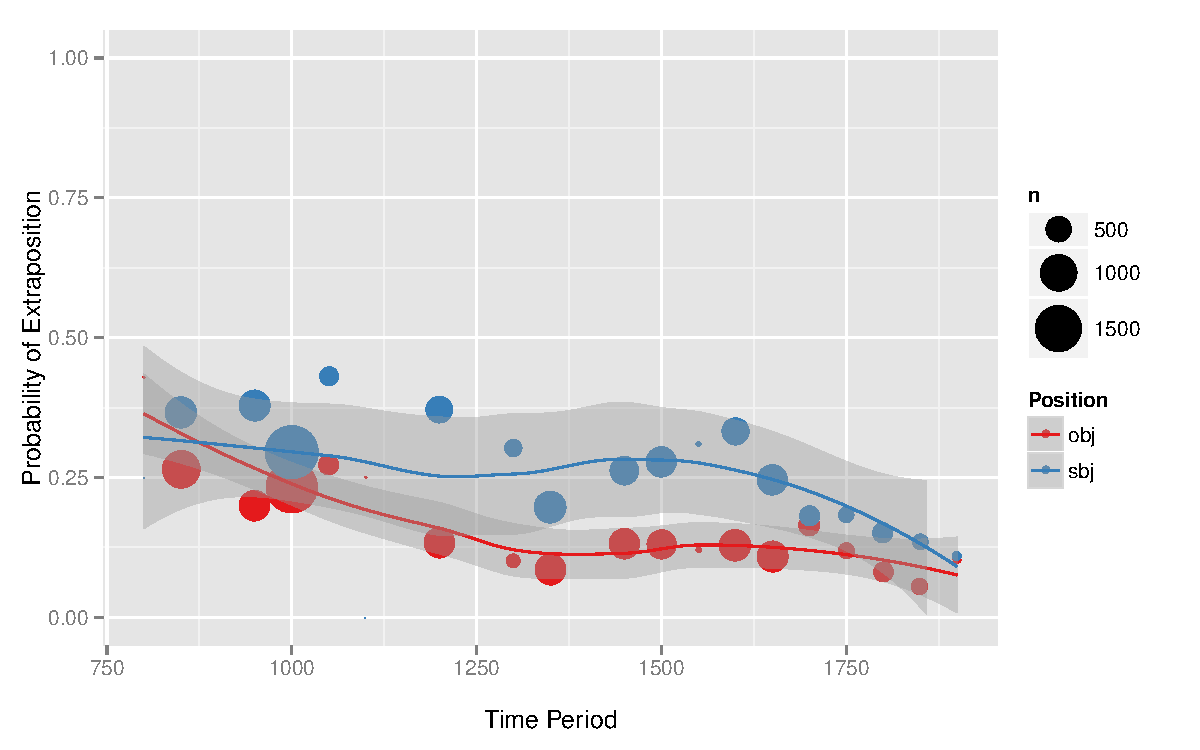
\includegraphics[width=1.1\textwidth]{stableVarTalks/exSbjObjYearBinned50Loessymeb.pdf}
\caption{Declining proportion of relative clause extraposition (vs. \textsl{in situ}), from early Old English prose through modern English. N = 18530 relative clauses. Lines are loess.}
\label{engfig}       % Give a unique label
\end{figure}

\begin{figure}

  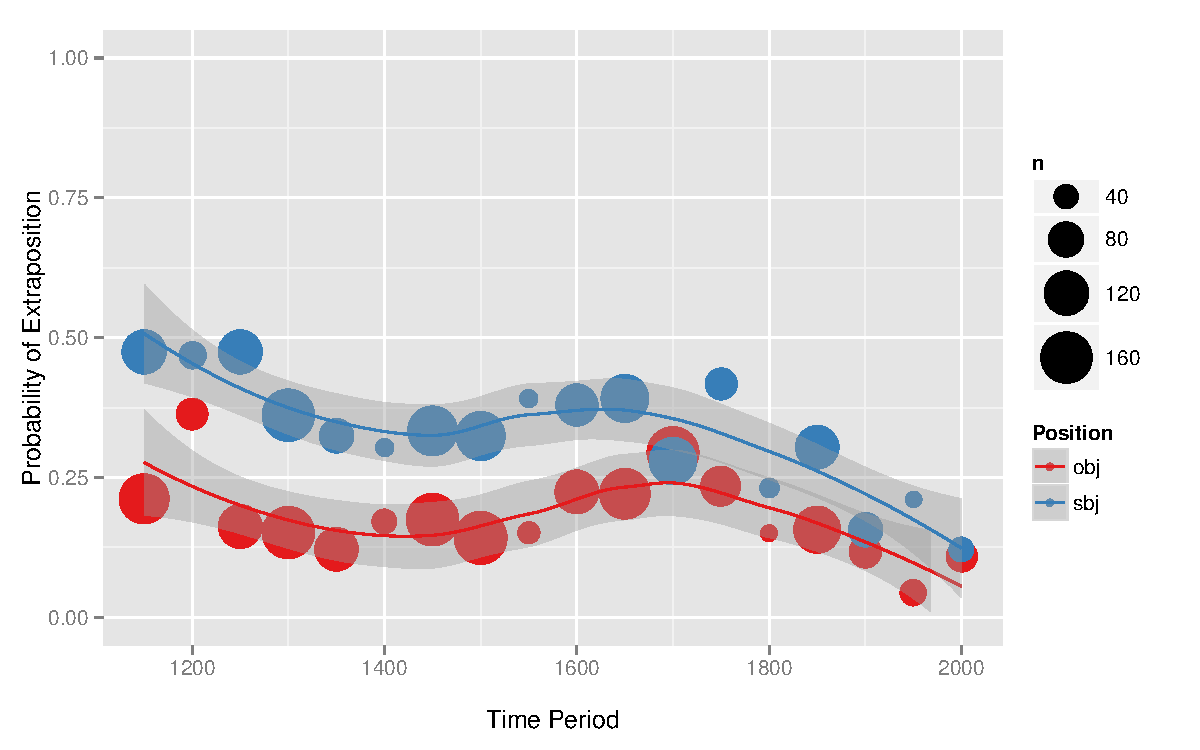
\includegraphics[width=1.1\textwidth]{stableVarTalks/exSbjObjYearBinned50Loessice.pdf}
\caption{Declining proportion of relative clause extraposition (vs. \textsl{in situ}) from subject and object positions, early Old Icelandic prose through modern Icelandic. N = 3486 relative clauses. Lines are loess.}
\label{icefig}       
\end{figure}

\begin{figure}
  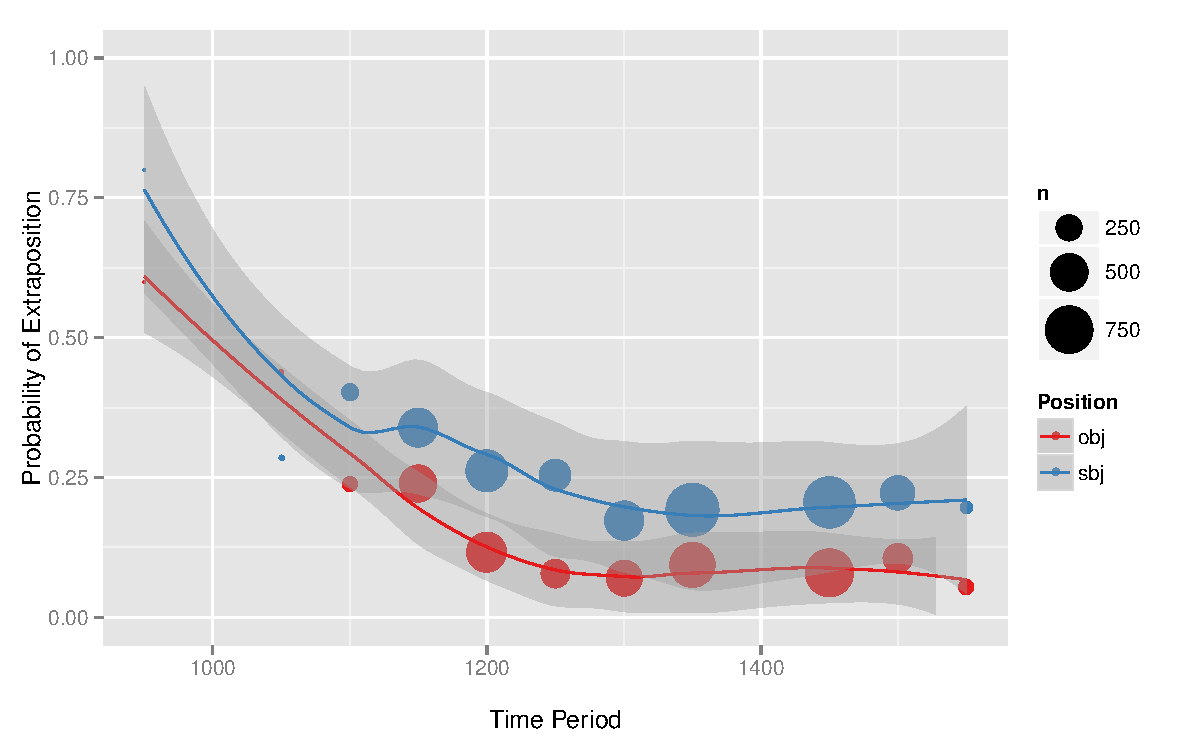
\includegraphics[width=1.1\textwidth]{stableVarTalks/exSbjObjYearBinned50Loessfre.pdf}
\caption{Declining proportion of relative clause extraposition (vs. \textsl{in situ}) from subject and object positions, Old and Middle French. N = 8207 relative clauses. Lines are loess.}
\label{frefig}       
\end{figure}

\begin{figure}
  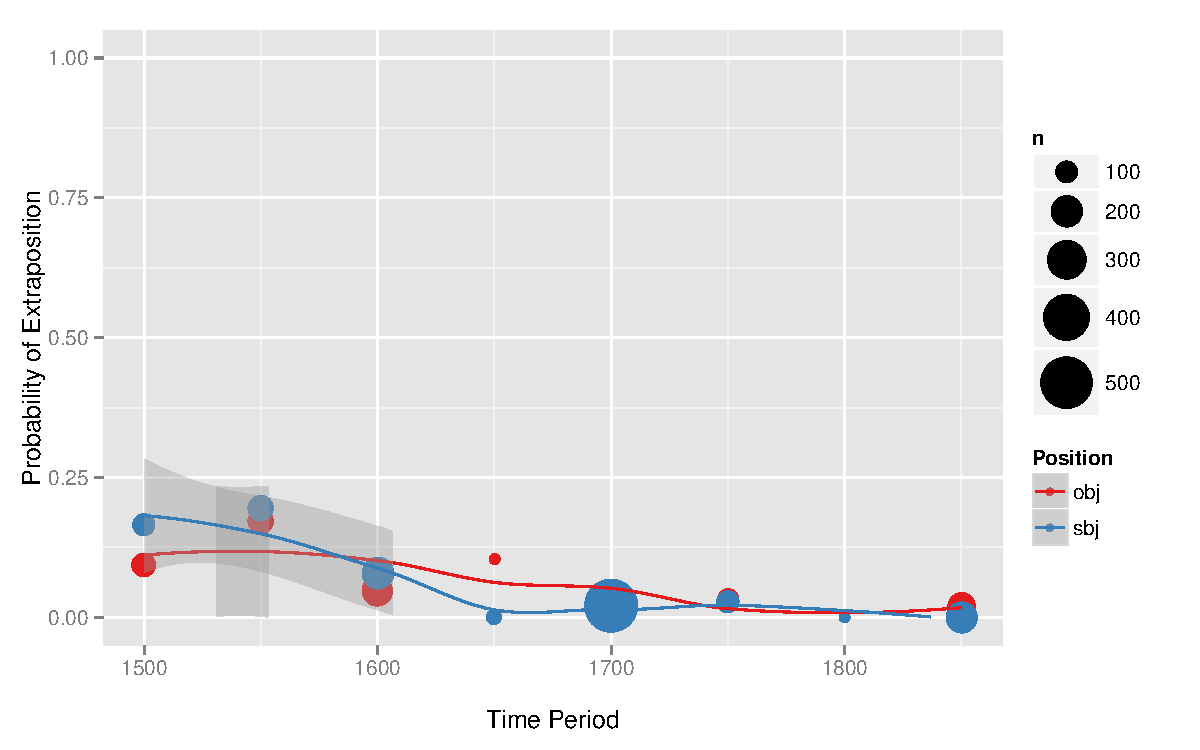
\includegraphics[width=1.1\textwidth]{stableVarTalks/exSbjObjYearBinned50Loessport.pdf}
\caption{Declining proportion of relative clause extraposition (vs. \textsl{in situ}) from subject and object positions, 15th-19th c. Portuguese. N = 2398 relative clauses. Lines are loess.}
\label{portfig}       
\end{figure}



As can be seen in the Figures for English (Figure \ref{engfig}) and Icelandic (Figure \ref{icefig}), the decline in extraposition is so slow that it could have been easily missed if the corpora of English (collectively) and Icelandic were not at sufficient time-depth (over 1000 years of data for each); any time-window of only a few hundred years would likely be too small to detect such a change at all.

For comparison, I conducted the same study on the Parsed Corpus of Early English Correspondence \citep[PCEEC][]{pceec}, which covers a period from the 15th through 17th centuries. The results of that study make the frequency of extraposition appear to be stable over time, shown in Figure \ref{pceecfig}.

\begin{figure}
  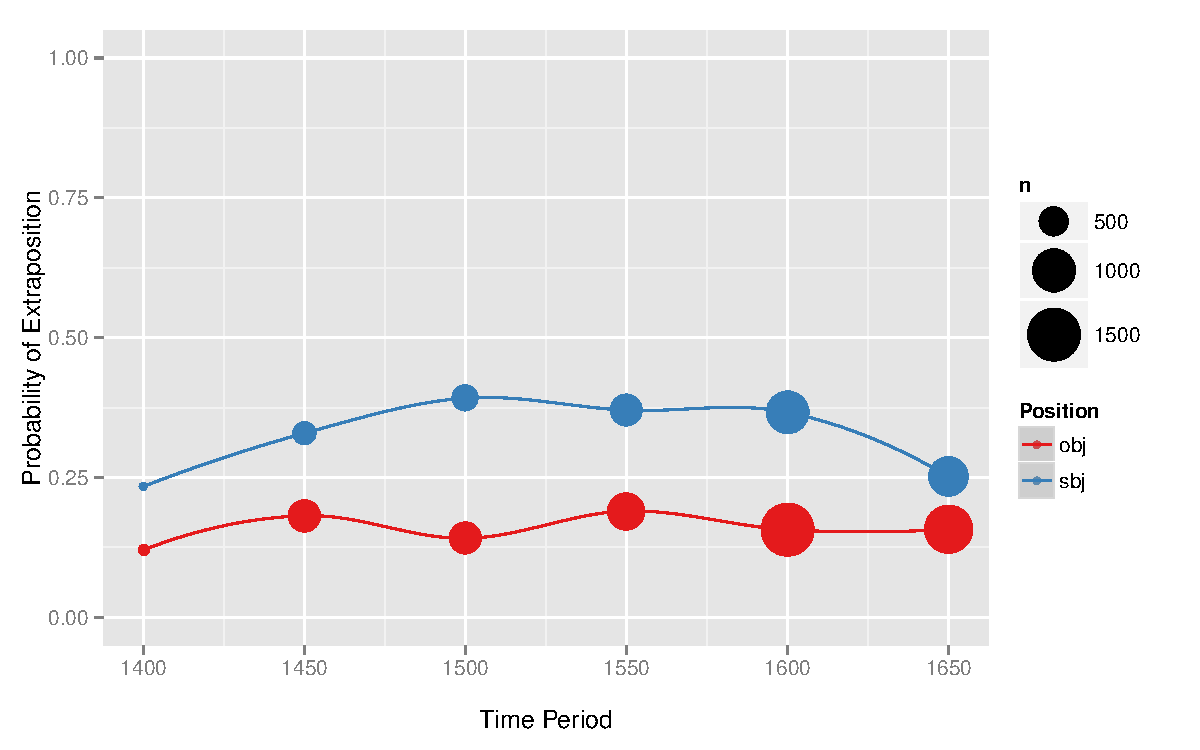
\includegraphics[width=1.1\textwidth]{stableVarTalks/exSbjObjYearBinned50.pdf}
\caption{Declining proportion of relative clause extraposition (vs. \textsl{in situ}) from subject and object positions, Parsed Corpus of Early English Correspondence. N = 8073 relative clauses. }
\label{pceecfig}       
\end{figure}

\noindent The results in Figure \ref{pceecfig} match the results from the larger English corpora for the same time period (compare Figure \ref{engfig}), but miss the change entirely; simply by accident, the 250-year time-slice of the PCEEC happens to not reflect the change, which then becomes visible once we observe a larger diachronic window.

Nevertheless, fitting a logistic regression model shows that the decline in extraposition is statistically significant in each of the languages; text year is a significant factor in the model, showing that an interaction between text year and extraposition significantly improves model fit (p < 0.00001 for all languages), controlling for all other possible interactions involving: matrix/subordinate clause-type, simple text vs. reported/quoted speech\footnote{Clauses containing quoted speech in the texts are annotated with a special tag in these corpora.}, subject vs. object position, and weight of the subordinate clause (i.e. length measured in number of words).

Interestingly, a model constrained to have the same slope parameter for the decline in both Icelandic and English (controlling for the same factors above) fits well, and not significantly better than a model which allows different slope terms for the two languages (p $\approx$ 0.45). This is reminiscent of the Constant Rate Effect \citep[][among others]{kroch1989, pintzuk1991, santorini1993a}, which states the different surface realizations of the same underlying linguistic object will change with the same slope as each other as that underlying linguistic object changes. Though the situation here is not one of comparing different linguistic contexts, but rather different populations of speakers (i.e. Icelandic and English), perhaps the same basic logic applies: the same trajectory of change could indicate that the same forces are underlying the change in both populations, both in terms of what is driving the change, and in terms of which basic linguistic object is undergoing change. 

However, any model which includes the French and Portuguese data fits significantly worse when it assumes the same slope for the change over time. This is true if French and Portuguese are modelled together, separately from Icelandic and English, or if any combination of languages including either French or Portuguese are modelled together (p $\leq$ 0.01 in all cases). This either means that these languages show a similar-looking, but ultimately different change (at least at the time points we are observing), or that some other feature of those data sets is obscuring what should be the same slope as in Icelandic and English. Since the text-sampling methods were designed to control for genre effects over time in the Icelandic and English corpora, but this was not done in the same way for the Tycho Brahe and MCVF corpora (and the latter is the only corpus which contains significant amounts of poetry as well as prose), we cannot rule out the possibility that the estimated slopes for French and Portuguese have been obscured by factors that are extraneous to the issue under investigation.

%, and genre (for IcePaHC only\footnote{Genre is easier to code for in the IcePaHC annotation. }


\section{Discussion}
\subsection{Extraposition As Competing Grammars}
\label{compete}

One consequence of the study above is that extraposition, which is usually described as an optional movement process producing multiple output options within a single grammar, is in fact behaving diachronically more like two co-existing linguistic objects, one replacing another over time just as in the classic cases of ``competing grammars'' \citep[][etc.]{kroch1989, kroch1994, santorini1992}. As \citet{kroch1994} discusses at length with respect to the ``Blocking Effect'' \citep[an expanded understanding of the principle first proposed in ]{aronoff1976}, situations of competing grammars are inherently diachronically unstable for general, cognitive reasons. In all four languages (with the possible exception of modern Portuguese), even though the loss of extraposition began at least a thousand years ago, the change is still in progress at the present time. Thus, the seeming optionality between extraposed and non-extraposed relative clauses is really most simply described as the code-switching that is characteristic of a change in progress (the definition of ``competing grammars'').

Once two structures (or two versions of a functional head, following the Borer-Chomsky conjecture; \citealt{borer1984, kroch1994}, so named in \citealt{baker2008}) are both available to a speaker with the same meaning or function, that is a situation of competition for language use: one of two possible forms is chosen by the speaker for use in a given utterance. As will become important later, this is true even if the two structures don't have exactly the same meaning, function, or context of use, but just overlap in meaning, function, or context of use; there will still be some context where the speaker is forced to choose between the two, putting them in competition for the finite resource of use, or speaker-time.

At this point, nothing more needs to be said in terms of grammatical apparatus in order to explain diachronic instability. Competition in use between functionally equivalent linguistic forms will be unstable diachronically by virtue of the fact that human brains prefer not to store or learn synonomous forms, whenever possible; indeed, this is probably a child language acquisition strategy, reducible to the independently observed ``Principle of Contrast'' \citep[][inter alia]{clark1987, clark1990}. In other words, competing syntactic forms is an unstable situation because they are subject to the same cognitive ``Blocking Effect'' as morphological doublets such as Middle English \textsl{lough, laughed} (laugh-\textsc{pst}; \citealt{taylor1994}), in the way suggested by \citet{kroch1994}.  (For much more discussion of the Blocking Effect and how it can be reduced to independent principles, see \citealt{fruehwaldwallenberginprep}.)

But this is only true under a simple, restrictive model of grammar: if the grammar is not specifically engineered to stably produce and maintain optionality as one of its design-features, then it won't. The grammar simply produces derivations by putting atomic pieces together, and if the brain needs to choose between two pieces for the same function at some point in the derivation, that creates apparent optionality on the surface, and also diachronic instability. If, on the other hand, a grammar is specifically designed to accommodate optional or stochastic processes as part of the derivation, such as Stochastic OT \citep{boersmahayes2001} or Noisy Harmonic Grammar \citep[][and much subsequent work]{boersmapater2008, pater2008}, the something additional needs to be said in order to explain the fact that even cases as close to diachronic stability as extraposition, are in fact changes in progress where one structure replaces another.

\subsection{Consequences for the Analysis of Relative Clause Extraposition}

This basic generalization stands regardless of the specific analysis one proposes for relative clause extraposition, and must be accommodated in any reasonable analysis: the diachronic instability means that somewhere in the derivation, the speaker makes a (probably unconscious) choice between two syntactic formatives that are functionally equivalent in many contexts.(Note that they need not be \textbf{entirely} functionally equivalent for change to be imperative: I return to this point in section \ref{slow}.) While various analyses could accommodate this generalization, there is currently an analysis of English relative clauses, proposed for independent reasons, that treats relative clauses as being in a state of competing grammars: \citet{sauerland2003}. Given the parsimony between Sauerland's independent arguments, the theory of competing grammars, and the empirical result above, I suggest the evidence lines up in favor of the Sauerland analysis of relatives. The loss of relative clause extraposition can then seen as the loss of Sauerland's ``matching'' type of relative, and the slow ascendency of the ``raising'' type of relative. This analysis of the change is not without problems, however, and I point out some of these, understanding that the data is not refined enough to answer them at this time.
%Revise last sentence, discuss Sauerland briefly, say how it implies competing grammars, then move on to culicover and rochemont after these examples:

\subsubsection{Competing Structures for Relative Clauses}

%FIX THIS TO BE LESS SURE ABOUT SAUERLAND, and STATE EXPLICITLY THAT IT MAY BE AN EXCURSIS

\citet{sauerland2003}, building on a proposal in \citet{carlson1977}, proposes that English relative clauses, are usually ambiguous between two possible structures. These two structures, the \textsl{matching structure} and the \textsl{raising structure}, are used inerchangeably in most cases, though their syntax is subtley different, and circumstances can arise that force a choice between them.\footnote{Sauerland's proposal is intended to resolve the longstanding controversy in the relative clause literature over whether relative clauses involved empty operator movement, as was standardly assumed in most treatments prior to \citet{kayne1994}, or whether they result from the NP ``head'' of the relative itself moving from the gap site inside the relative clause.} According to Sauerland, the raising structure is one along the lines of \citet{kayne1994}'s analysis, where the ``head'' of the relative clause is moved from a position internal to the relative clause, as I schematize below in (\ref{sauerStruc1}), and then the D heading the DP containing the relative clause takes a clausal complement, rather than an NP complement (shown as ``FP'' below just because I'm not committed to the particular version of the split-CP hypothesis one adopts to make this analysis work). The matching analysis has a similar structure internal to the relative clause, but with ellipsis of the NP rather than movement of the NP to Spec(FP), as in (\ref{sauerStruc2}) below.

\begin{exe}
    \ex \label{sauerStruc1} \Tree [.DP {D\\a} [.FP {NP_j\\book} [.F' F [.CP [.DP_i {D\\which} {NP\\\textsl{t_j}} ] [.C' C \qroof{Kim read \textsl{t_i}}.TP ] ] ] ] ]
    \ex \label{sauerStruc2} \Tree [.DP {D\\a} [.NP {NP\\book} [.CP [.DP_i {D\\which} {NP\\\st{book}} ] [.C' C \qroof{Kim read \textsl{t_i}}.TP ] ] ] ]
\end{exe}

\noindent For the matching-type relative, Sauerland does assume that the relative clause modifies an NP ``relative head'', which is its own constituent outside the relative clause. Though he doesn't give the details of how the relative relates syntactically to the upstairs NP, I'll assume the relative clause is right-adjoined to the NP in the upstairs clause, as in the classical analysis of relative clauses (as I show in \ref{sauerStruc2}). This is in contrast to the raising-type relative in (\ref{sauerStruc1}), in which the relative clause is itself the complement of D. I've shown this in the structures above.

Sauerland's analysis is actually a competing grammars analysis of relatives, though he does not use that term. Combined with the hypothesis presented above, his analysis predicts that there should some sort of change in progress in relative clauses. Note that the matching-type of relative is entirely compatible with relative clause extraposition, as it adjoins freely to maximal projections. As with other kinds of modification, the only restriction as to where it adjoins is that it must be interpretable in its adjoined position; it must be interpreted with respect to some antecdent ``relative head'' NP, and in Sauerland's account, trigger ellipsis of the NP. This is very similar to \citet{culicoverrochemont1990}'s analysis of relative clause extraposition, where it doesn't involve movement \textsl{per se}, but rather choice of adjunction sites for the relative clause, and a structural restriction on how far the relative can be from a potential antecedent. In fact, the locality restriction on interpretation that Culicover and Rochemont propose probably makes more sense as a restriction on ellipsis. Thus, the matching relative is an adjoined modifier with some limited freedom of adjunction.

Sauerland's raising-type relative, on the other hand, is incompatible with extraposition, and so the loss of relative clause extraposition can be viewed as a side-effect of the gradual out-competition of the matching structure by the raising structure. First, \citet{baltin2006} lists a number of problems with accounting for extraposition under the raising analysis, which would apply to raising-type relatives under Sauerland's analysis. A full discussion of these issues is beyond the scope of this article, but suffice it to say that the challenges Baltin catalogues for the raising analysis fall away if there is another possible structure, the matching structure, which can accommodate extraposition as simply an additional adjunction site.

Secondly, there is independent evidence from binding that extraposed relatives are always matching relatives. Sauerland discusses a number of binding examples which are only grammatical under one or the other structure, and so force a particular structure to emerge in the mind of the speaker. Among these are Condition A, which forces the raising structure when an anaphor inside the relative head is bound by a DP inside the relative clause; such sentences can only be grammatical if the NP containing the reflexive has raised from inside the relative, and so can reconstruct and be bound in that position. Similarly, Sauerland discusses variable binding, where a quantifier inside the relative can only bind a variable inside the relative head NP if the NP can reconstruct to a position inside the relative. Examples of these two with relative clauses \textsl{in situ} are shown below in (\ref{prinAsitu}) and (\ref{boundVarSitu}). 

Sauerland claims that when the Principle A and quantifier binding are not possible in a sentence, it is because only the matching analysis is available, and so the necessary reconstruction cannot take place. Note that the extraposed versions of (\ref{prinAsitu}) and (\ref{boundVarSitu}), namely (\ref{prinAex}) and (\ref{boundVarEx}) are ungrammatical. (I've also included parallel examples of extraposition without the binding in (\ref{control1}) and (\ref{control2}), just to show that there's no independent problem with extraposition in these examples.) \footnote{Note that the examples below all contain demonstratives in the DP containing the relative, or which the relative is interpreted with respect to. This is because, as Sauerland discusses, the raising analysis is not possible inside a DP headed by an indefinite determiner. He suggests that this may be true for all indefinites, though the data is not clear (see his footnote 9). In order to avoid this confound, I have avoided indefinites in my examples, but extraposition is degraded from definite DPs \citep[][and references therein]{baltin2006} unless they are headed by a demonstrative. I am tempted to suggest that the fact that extraposition is degraded from definite DPs somehow relates to the presence of the raising analysis in exactly these cases, but I don't feel the data on definiteness and matching vs. raising is clear enough to make such a claim at present, particularly since the binding facts show that the matching structure is available \textsl{in situ} in definite contexts.}

\begin{exe}
                  
    \ex \begin{xlist}
         \ex \label{prinAsitu} That picture of himself that John likes a lot was just published.
         \ex \label{prinAex} ?* That picture of himself was just published that John likes a lot.
                  \end{xlist}
                  
              
   \ex \label{control1} \begin{xlist}
         \ex \label{controlAsitu} That picture that John likes a lot was just published.
         \ex \label{controlAex} That picture was just published that John likes a lot.
                  \end{xlist}
%         \citep[Adapted from][23]{culicoverrochemont1990}
         
%        \begin{xlist}
%         \ex \label{prinAsitu2} The picture of himself which Chomsky likes appeared online.
%         \ex \label{prinAex2} The picture of himself appeared online which Chomsky likes.
%         \end{xlist}
 
 %\ex \label{idiom} The headway John made proved insufficient\\
% (from \citealt{sauerland2003}: 212)
 %\ex \label{idiom2} The tabs which the FBI kept on Malcolm X weren't very useful.
 %\ex \label{idiomComp} The newspaper stories were terrible 
  
  \ex \begin{xlist}
        \ex \label{boundVarSitu} That draft of her paper that every student produced at the beginning of the semester was also graded.
         \ex \label{boundVarEx} *? That draft of her paper was also graded that every student produced at the beginning of the semester.
%         \ex \label{boundVarSitu} At least one article of hers that every academic is actually proud of has been published.
%         \ex \label{boundVarEx} At least one article of hers has been published that every academic is actually proud of.
 \end{xlist}    
 
\ex  \label{control2} \begin{xlist}
        \ex \label{controlSitu} That draft of the paper that the students produced at the beginning of the semester was also graded.
       %  \ex  The draft of the paper that every student had at the end of the semester was graded.
       \ex \label{controlEx} That draft of the paper was also graded that the students produced at the beginning of the semester.

%         \ex \label{controlEx} The draft of the paper was graded that every student had at the end of the semester.
%         \ex \label{controlSitu} At least one article that every academic is actually proud of has been published.
%         \ex \label{controlEx} At least one article has been published that every academic is actually proud of.
  \end{xlist}  
         
    
         
 %        \citep[Adapted from][]{thomsheycock2014}
%  \begin{xlist}
%         \ex \label{prinBex} A picture of him appeared online which Chomsky painted/likes.
%         \ex \label{prinBsitu} A picture of him which Chomsky painted/likes appeared online.
%         \end{xlist}
         
\end{exe}

\noindent The parallel examples with potential Principle C violations, however, are grammatical, as they should be under the matching structure:

\begin{exe}
    \ex That picture of John was just published that he likes a lot.
    \ex That draft of Mary's paper was also graded that she produced at the beginning of the semester.
\end{exe}


The fact that the binding in three examples become ungrammatical under extrapostion shows that the reconstruction required for the binding cannot take place in an extraposed relative. This fact is consistent with the idea that extraposition necessarily involves a matching structure, and cannot contain a raising structure. The reconstruction thus cannot take place because the NP in the relative head, which needs to be bound, has never moved.

Given that extraposition always involves the matching structure, but the \textsl{in situ} relatives are in a state of variation between the matching and raising structures, then the loss of extraposition could be due to the replacement of the matching structure by the raising structure in general. If the speaker's syntactic apparatus makes the decision on which structure to use before or simultaneously with the decision to extrapose, then the gradual replacement of matching by raising will result in less extraposition over time. It would be elegant if the change could be described so simply. It would also be in line with the view I mentioned in section \ref{compete}, that grammar competition is really competition between multiple versions of a functional head, in this case, the D selecting either an NP or a CP. If this were always true, then it would be evidence for the Borer-Chomsky Conjecture. Unfortunately, there are also some shortcomings of the matching vs. raising approach to the historical facts in this case.

This analysis of the diachronic change has four potential problems. First, speakers may be able to choose the matching structure \textsl{in order to} extrapose. If this were the case, then even if raising replaces matching in the \textsl{in situ} case, the historical result should be that raising becomes specialized for the \textsl{in situ} case, while matching becomes specialized for the extraposed case, and some other factor would have to explain the loss of extraposition. It's hard to say if this specialization has taken place, since only matching is compatible with extraposition, but both analyses are currently compatible with the \textsl{in situ} position. Secondly, Sauerland (and references therein) observes that the raising structure is degraded in indefinite contexts, which is also where extraposition occurs most naturally. Thus, raising replacing matching would have little effect on the rate of extraposition (unless this is actually one of the reasons the change is so slow). Thirdly, since the matching structure can occur in more contexts than the raising structure can (i.e. indefinites and extraposition), there might be more evidence to the learner for matching than for raising. According to models like \citet{yang2000}, this should result in matching winning the competition over time, rather than losing it. And there is a fourth problem, which I discuss below.


\subsubsection{A Wrinkle: Competing Adjuction Sites}

If we accept Sauerland's analysis of relatives as involving two structures, a raising structure and an adjoined matching structure, then extraposition can be straightforwardly analyzed as an instance of the matching type. Since this type presumably adjoins in the way a modifier does, I will adopt \citet{culicoverrochemont1990}'s conclusion that (matching) relatives adjoin to any maximal projection where they can receive an interpretation, and there is a general principle (their ``Complement Principle''\footnote{The name is historical: their proposal does not apply only to complements.}) governing possible antecedents for the matching relative. If we combine the approaches of \citet{culicoverrochemont1990} and \citet{sauerland2003}, then this principle becomes a constraint on the ellipsis of the ``matched'' NP. According to this view, the extraposed version of the relative clause in (\ref{crex}) is not derived by movement, but rather represents an alternative adjunction site for the relative, higher up the in structure.

%\footnote{In fact, the generalization may be that the relative clause can be adjoined either inside the DP, or within the $v$P phase. If this is correct, then \citet{culicoverrochemont1990} and Sauerland's constraint on ellipsis of the matched NP could be recast in terms of phase theory: the ``Complement Principle'' can be reduced to a requirement that the relative clause be sent to LF for interpretation on the same phase as the matched NP. But the details of such a proposal are beyond the scope of the present article.}

\begin{exe}
    \ex \begin{xlist}
         \ex \label{crinsitu} A man that no one knew came into the room.
         \ex \label{crex} A man came into the room that no one knew.
         \end{xlist}
         \citep[][23]{culicoverrochemont1990}
\end{exe}

Under this analysis, matching relatives are modifier CPs which can adjoin in at least two positions in the phrase structure, without interpretive difference. This creates a situation of competing grammars, even if both adjunction sites are hosting instances of the matching structure. According to the definition of competing grammars I gave above in section \ref{compete}, any situation where multiple structures are available to a speaker in the same context, there is competition for use between the two structures. Even though an extraposed relative is not equivalent to an ``\textsl{in situ}'' relative in all ways (especially prosodic, as I discuss below in \ref{slow}), there is still overlap in use: there are still situations where a well-formed utterance can be produced with either the extraposed or the non-extraposed variant. In this area of functional overlap, a speaker is nonetheless forced to choose one or the other, and this competition in use should be diachronically unstable according to the theory I've laid out above, following \citet{kroch1994}.

By hypothesis, this situation of competition means that even within the matching structure, there is potentially diachronically unstable variation. The two adjunction positions are in competition within the matching structure, independently of the competition between the matching and raising structures (which also exists, if \citealt{sauerland2003} ). This means that the loss of extraposition could be the gradual ascendancy of the raising structure, as I suggested above, or it could be the ascendancy of the low, NP-adjunction position within the matching structure. Even if the raising vs. matching competitoin is indeed taking place, this additional variation would still exist, and could alone be the diachronic loss of extraposition. It could even be the case that the raising vs. matching competition is resolving in some other way, e.g. matching could be winning over raising, but the low adjunction site is winning over the high one within matching, leading to the loss of extraposition.

The high adjunction vs. low adjunction view of the change is much more difficult to see as competition between functional heads, as \citet{kroch1994} suggests based on the Borer-Chomsky Conjecture. But this really highlights a problem with the very idea of any phrases freely adjoining to multiple sites in the phrase structure, and indeed with the idea of syntactic optionality in general: if a derivation is an algorithm, a sequence of functions to be applied to an input, then if the output of one of those functions is indeterminate the derivation will simply never converge on an output. (It would actually be an ill-defined function, mathematically.) Optionality, including multiple adjunction sites, can anly mean that there are two possible derivations, one employing e.g. Function 1 (or Head 1), and the second employing Function 1' (or Head 1').

So, perhaps the best way to understand the variation in relative clause structures is to view it as a 3-way competition between one raising structure, which is always ``\textsl{in situ}'', as it contains the relative head, and two matching structures, each of which specify either low adjunction or high adjunction. It could also be that adjunction is the wrong description of the modification relation, and that the CP is actually hosted by a silent modifier head, but a different version of the head for high attachment to the main clause then for low. (A full discussion of the details of this possibility would be beyond the scope of this article.) In either case, it is the high-attached relative clause that is the adjunction case, losing out in its competition with two ``\textsl{in situ}'' structures. It will be the subject of future work to more carefully determine whether there really is a 3-way competition here.

%Prediction: You should be able to get a raising clause inside a matching but not the other way round.

Since the competition between adjunction sites for relative clauses (if that is the right way to view the two positions), in the Culicover and Rochemont sense, is most likely a necessary part of how and why the loss of extraposition takes place, I'll continue the rest of the discussion in this article in terms of competition between adjunction sites. This is not to dismiss the idea that the raising vs. matching structure competition may also be implicated in the change, but merely to say that it is unlikely to be the entire story of the change for the reasons I give above, and that distinguishing the 2-way vs. 3-way competition scenarious will be the subject of future work.

\subsection{Why So Slow?}
\label{slow}

At this point in the discussion, readers are likely to have in a mind an obvious criticism of the proposal in section \ref{compete}, that extraposed and non-extraposed variants are in competition for speaker use (whether we think this is due to matching vs. raising, or competition between adjunction sites within the matching structure). It is well-known that the extraposed and \textsl{in situ} relative clause variants are not really functionally equivalent, as extraposition is more likely to occur if the relative clause is prosodically heavier.\footnote{Of course, I am not claiming that prosodic weight is the only factor which affects the probability of extraposition, but the existence of other effects does not detract from the main point we are making.} Indeed, this is a crucial point, because it is this specialization of the two variants for different prosodic weights which accounts for the exceedingly slow speed of this change: the functional difference between the two variants removes much of the competition between then, because it keeps at a minimum the contexts in which the two overlap in use. However, the specialization does not remove \textbf{all} of the overlap in use, so the competition still exists, and the change still continues.

The specialization of the two variants for different prosodic weights can never be complete, in fact, because extraposed vs. \textsl{in situ} is a categorical (binary) variable, while prosodic weight is a continuous one. For a full discussion of this complex and interesting issue, I refer the reader to \citet{fruehwaldwallenberginprep} where this and other cases are discussed in much greater detail, and a full theory of linguistic specialization is developed \citep[see also][]{fruehwaldwallenberg2013, wallenberg2013b}.

For the present discussion, I will just briefly mention one result which is also presented there. A study of individual authors in the PCEEC shows that their probability of extraposing a given relative clause from subject position depends on the prosodic weight of the relative clause (measured in number of words), and does so in a continuous manner: as the number of words increases incrementally, so does the probability of extraposition. For instance, speakers do not split the weight dimension into categories of ``heavy'' and ``light'', so that it matches the binary dimension of extraposition, but rather allow extraposed and non-extraposed tokens to fall along the entire scale. This is shown for the systems of individual PCEEC authors in Figure \ref{pceecWeight}.\footnote{Only authors with 100 tokens or more of relative clauses were included.}

%Cite other paper with Joe

\begin{figure}
  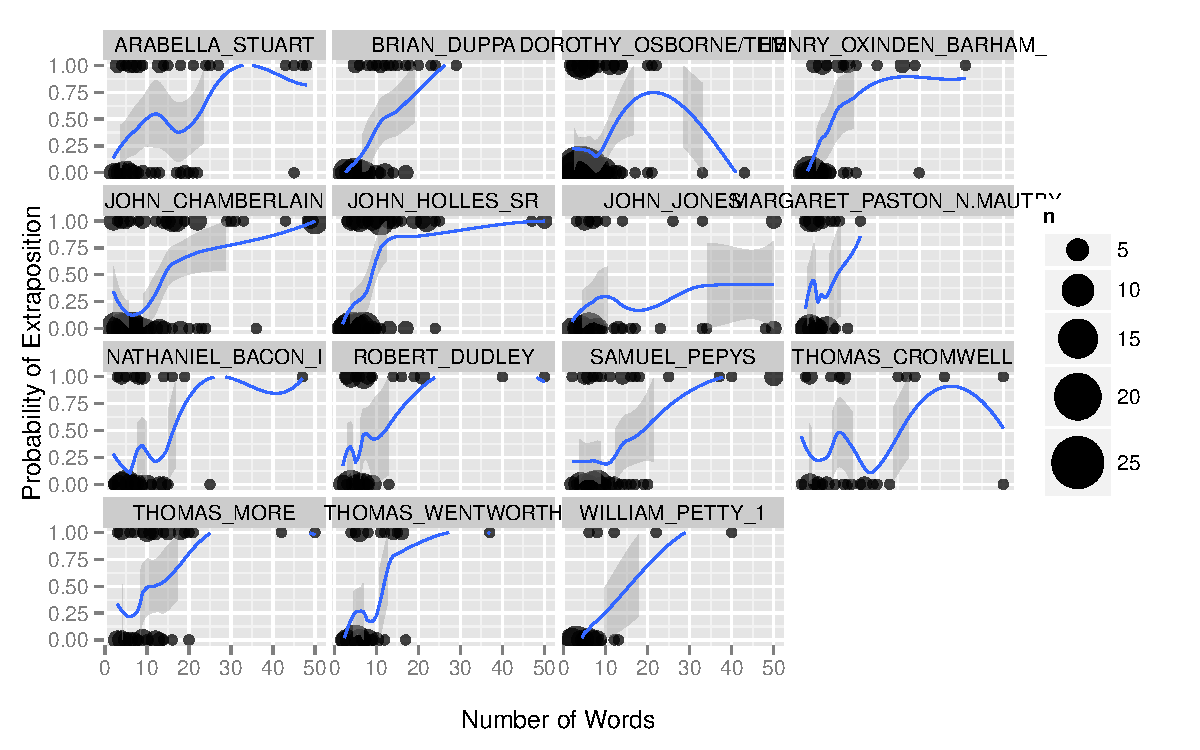
\includegraphics[width=1.1\textwidth]{stableVarTalks/exSbjWeightLoess.pdf}
\caption{Effect of prosodic weight on the probability of relative clause extraposition from subject position, for individuals in the Parsed Corpus of Early English Correspondence. Lines are loess.}
\label{pceecWeight}       
\end{figure}

To summarize, because the extraposed and \textsl{in situ} relative clause variants have specialized for different contexts (different prosodic weights), a large amount of the competition between them in use has been removed, and so the replacement of one by the other has slowed considerably. However, because the domain of specialization is continuous, the two variants are unable to specialize completely, and so some of the competition remains. Thus, the extraposed variant continues to be lost over time, but very slowly.

\subsection{Origin of Relative Clauses}
\label{pie}

The next portion of this article is by far the most speculative, as suggestions regarding the actuation of a particular linguistic change often are. Nevertheless, it may be interesting to explore some implications of the very slow rate of change shown in the data above. The change is slow enough that it may well have been in progress for some thousands of years, and so quite possibly predates the differentiation of some of the languages under investigation into mutually unintelligible varieties. In particular, it may be the case that the change in extraposition relates to the origins of Indo-European relative clauses, and that the change actually began when relative clause embedding was first innovated in Indo-European.

If we follow the non-movement adjunction analysis of relative clause extraposition in \citet{culicoverrochemont1990}, then the ``extraposed'' version of a relative clause is actually the historical form of all Indo-European relative clauses, and the ``\textsl{in situ}'' version is a later innovation. \citet{kiparsky1995}, following a number of previous researchers (see his references), proposes that relative clauses in Proto-Indo-European (PIE) only existed as clausal adjuncts; they were not truly embedded within the matrix clause, forming a constituent with some NP within it, but rather were adjoined to the matrix clause and associated semantically with some NP element within it.\footnote{Kiparsky's analysis is broadly compatible with theories positing an historical stage prior to this one in which there were not even adjoined relative subordinate clauses without gaps, but paratactic main clauses which were later reanalyzed as subordinate clauses \citep[e.g.][]{haudry1973}. However, Kiparsky's analysis certainly does not depend on there being such a stage.} I will assume that the high, ``clause-adjoined'' relatives that Kiparsky describes could represent TP- or CP-adjunction, and some could be $v$P-adjoined (though this is often difficult to determine)\footnote{Relatives appearing at the right edge of the clause are often ambiguous between these positions. Correlatives, high-adjoined on the left in languages like Sanskrit, may always be TP-adjoined, but this also depends on whether one adopts an analysis of head-final clause structures which is underlyingly head-final. Left-adjoined correlatives could be $v$P-adjoined under an analysis of head-final clause structures as underlyingly head-initial, but with ``roll-up'' movement of $v$P to Spec(TP), as in \citet{biberauer2003} and \citet{wallydiss}. In either case, though, there will still be an asymmetry between the syntax of left-adjoined and right-adjoined high relatives, but I leave a full discussion of this issue as a topic for further research. See also the following footnote.}; these are the possible adjunction positions for ``extraposition'' I mentioned above in section \ref{compete}, with regard to Culicover and Rochemont's analysis.\footnote{I will here note a problem for my analysis, pointed out by an anonymous reviewer: the high-adjoined relatives of the Old Indo-European languages are often left-adjoined correlatives, as in (\ref{vediccar1}), rather than clause-final and right-adjoined, as I am arguing for the modern extraposed relatives. If the old correlative/high-adjoined system is really the same system as modern extraposed relatives, then there is a step missing from my story: when and why did the left-adjoined relatives disappear? I do not currently have a complete answer to this, and it may be a point against the analysis presented here. However, it may also be that the left-adjoined relatives have remained syntactically possible throughout the histories of the languages in question, but once high-adjoined relatives began to specialize for prosodic heaviness, the prosodic systems of early Romance and Germanic increasingly required heavy relatives to appear clause-finally. In the modern languages, the prosodic specialization ensures that left-, high-adjoined heavy correlatives should occur with a probability near zero.} These high-adjoined relatives represent either the only attested system or the dominant system found in various Old Indo-European languages, such as Sanskrit, Hittite, Old Latin (\citealt[][155]{kiparsky1995}, and references cited therein). According to Kiparsky, the low-adjoined relative clause (again, following an adjunction analysis), the \textsl{in situ} variant which appears within a DP, is a later innovation, and comes to be the dominant form in Germanic, as that family differentiates from the rest of PIE (presumably this would apply to Romance as well).

Although Kiparsky only discusses the earliest and latest stages of the change, not the detail of how the change progressed in the interim, it is straightforward to apply our understanding of syntactic change in progress to this case from other changes that have been studied in quantitative detail (going back to \citealt{kroch1989}, \citealt{santorini1989}). Starting from a Sanskrit-like system of clause-adjoined ($v$P-adjoined) relative clauses, as Kiparsky suggests, once a new, DP-embedded type of relative clause is innovated, it will come into competition for use with the old clause-adjoined system. This would create the kind of variation we have observed in all four languages, if we accept that ``extraposition'' is actually just the remnant of the old clause-adjoined relative system. Then, in order for the DP-embedded system to become dominant, as Kiparsky suggests it has in Proto-Germanic, the DP-embedded (``\textsl{in situ}'') variant would have to spread at the expense of the clause-adjoined (``extraposed'') variant over a number of generations. This is exactly the historical progression I have shown above (with the addition that the change was slowed by specialization for prosodic weight, as I have already discussed).

The idea that the high/clause-adjoined relative system has never really left Germanic and Romance, but is really simply the ``extraposed'' variants (following \citealt{culicoverrochemont1990}) is supported by the fact that clearly clause-adjoined relatives are still possible in languages like modern English and modern Icelandic. Kiparsky argues that in cases such as the Vedic Sanskrit sentence in (\ref{vediccar1}), where the ``head'' of the relative is contained inside the relative clause and the main clause contains a different ``head'' to which the relative refers, the only possible analysis is the clause-adjoined one.

\begin{exe}

\ex \label{vediccar1} \gll yó mártya\d{h} śíś\={i}te áty aktúbhir m\={\'{a}}, na\d{h} sá ripúr \={i}śata \\
which mortal sharpen-Mid-Sg overly nights-\sc{instr}, not us-\sc{gen} that trickster dominate-Subj3Sg\\
\quad ``As for the mortal who makes himself too sharp by night, may that trickster not gain power over us''\\
\citep[RV 1.36.16, cited in][156]{kiparsky1995}
\end{exe}

\noindent The same is true for the 19th century English example in (\ref{engcar1}) and 20th century English example in (\ref{engcar3}). (Note that the same construction would be grammatical in 21st century English.)

\begin{exe}
         \ex \label{engcar1} By God's blessing I calculate that the Spirit of Dishonesty shall not get dominion over me; nor the Spirit of Despondency, nor any other evil spirit; in which case
all will and must be well.\\
(Letter by Thomas Carlyle, date: 1835; ID CARLYLE-1835,2,266.176 in PPCMBE)
        \ex \label{engcar3} Nowadays, however, flowers can be arranged in various styles -- some flat, some slightly raised, some bunched boldly in certain
places and forming the piece de resistance of
the whole work -- all of which variations depend upon the artistic
perceptions of the operator.\\
        (\textsl{Commercial gardening...}, date: 1913;ID WEATHERS-1913,1,9.217 in \\PPCMBE)
\end{exe}

\noindent Similarly, the high-adjoined system is also evidenced by cases where the relative clause refers to the entire proposition, and is, in the words of \citet[][157]{kiparsky1995}, ``unlinked to any argument/modifier position'' in the main clause, as in the modern Icelandic and English examples in (\ref{icecar2}) and (\ref{engcar2}) respectively, or the Middle French one in (\ref{frecar}):

\begin{exe}
         \ex \label{icecar2} \gll hann hafði enn hvorki boðið mér vott né þurrt, sem var óvenjulegt á þeim bænum\\
         he had still neither offered me wet nor dry, which was unusual in that town.\\
         \quad ``he had still not offered me a drink, alcoholic or non-alcoholic, which was unusual in that town.''
         (\textsl{Ofsi}, date: 2008; ID 2008.OFSI.NAR-SAG,.485 in IcePaHC)
         \ex \label{engcar2} [if a man] sees a certain amount of his colleagues socially --  which is absolutely essential to general harmony...\\
         (\textsl{The schoolmaster...} ,date: 1908; ID BENSON-1908,73.313 in PPCMBE)
         \ex \label{frecar} \gll Ma Sibile, je vous ai escrit il n i a que deux jours, qui m anpaichera de vous inportuner de long discours \\
         My Sibile, I you-\sc{dat} have written there \sc{neg} it-\sc{dat} have but two days, which me prevents from you bother of long discussion\\
         \quad ``My Sibile, I wrote to you only two days ago, which prevents me from bothering you with a long discussion''\\
         (letter by Marguerite de Valois, date: 1573-1596; \\ID 158X-VALOIS-AUTOGRAPH-P,124.838 in MCVF corpus)

\end{exe}


Thus, this study has been able to build on Kiparsky's argument that the older, PIE system, consisted of high/clause-adjoined relatives, but I see no reason to conclude that they have disappeared from modern Germanic or Romance, nor that extraposed relative clauses are a separate phenomenon from the high/clause-adjoined system. Rather, accepting \citet{culicoverrochemont1990}'s analysis of extraposition as adjunction suggests a natural historical continuity: extraposition is simply the remnant of the older relative clause system (clause-adjoined), which has been in competition with the new, DP-internal relative clause system for well over a thousand years. But just as Kiparsky suggested, the quantitative study above does show that the old system is dying out, albeit very slowly.


\section{Conclusions}


This paper has shown that relative clause extraposition is in decline in four Indo-European varieties, and that the decline represents a previously undescribed class of language change. The change is a remarkable case in that the two variants have specialized for different functions, but this specialization has been incomplete due to the mathematical character of the domain of specialization. For this reason, the \textsl{in situ} relative system continues to replace the extraposed variant, but the change has slowed to a speed which is barely detectable. Fortunately, with diachronic parsed corpora of sufficient time-depth, it is possible to observe the change, and see that it is still in progress at the present date in all four languages.

The fact that the change is still in progress has implications for the analysis of relative clause extraposition. I have suggested that the best analysis of relative clause extraposition, in the light of the diachronic facts, is simply as an alternative adjunction position for relatives, in the spirit of \citet{culicoverrochemont1990}: interpreted lower but not moved from a matrix-clause-internal position. The high(er)-adjoined clauses have been in competition with ``\textsl{in situ}'' relatives for a very long time. This analysis has the additional benefit that it follows nicely from \citet{kiparsky1995}'s argument that all Proto-Indo-European relative clauses were matrix-clause-adjoined, and lower relatives are an innovation. This suggests that the decline in extraposition could have begun as a result of the innovation of lower ``\textsl{in situ}'' relatives in Indo-European. In that case, this is the oldest change in progress yet reported.



%Further questions: evidence to the learner in favor of matching or raising? Competition between adjunction sites? Specialization of matching and raising for indefinite and definite, respectively? Or is this actually an advantage for the 



%
% For two-column wide figures use
%\begin{figure*}
% Use the relevant command to insert your figure file.
% For example, with the graphicx package use
%  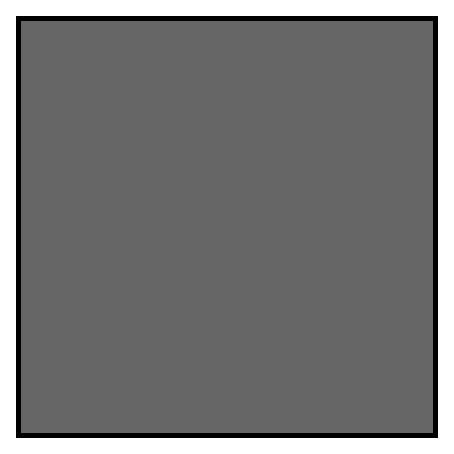
\includegraphics[width=0.75\textwidth]{example.eps}
% figure caption is below the figure
%\caption{Please write your figure caption here}
%\label{fig:2}       % Give a unique label
%\end{figure*}
%
% For tables use
%\begin{table}
% table caption is above the table
%\caption{Please write your table caption here}
%\label{tab:1}       % Give a unique label
% For LaTeX tables use
%\begin{tabular}{lll}
%\hline\noalign{\smallskip}
%first & second & third  \\
%\noalign{\smallskip}\hline\noalign{\smallskip}
%number & number & number \\
%number & number & number \\
%\noalign{\smallskip}\hline
%\end{tabular}
%\end{table}


%\begin{acknowledgements}

%\end{acknowledgements}

% BibTeX users please use one of
%\bibliographystyle{spbasic}      % basic style, author-year citations
%\bibliographystyle{spmpsci}      % mathematics and physical sciences
%\bibliographystyle{spphys}       % APS-like style for physics
\bibliographystyle{linquiry2} %use spbasic for journal of comparative gmc linguistics, etc.
\bibliography{joelrefs}   % name your BibTeX data base

%\section*{Appendix}

\end{document}
% end of file template.tex

 